% !TEX root = main.tex
\vspace{-0.4cm}
\section{The \linearpartition Algorithm}
\vspace{-0.1cm}


\newcommand{\pluseq}{\mathrel{+}=}


We denote $\vecx\!=\!x_1 ... x_n$ as the input RNA sequence of length $n$, and $\mathcal{Y(\vecx)}$ as the set of all possible secondary structures of $\vecx$.  
% $\vecy$ is a secondary structure 
% of $\vecx$ 
% in $\mathcal{Y(\mathbf x)}$. 
The partition function is: % $Q(\vecx)$ 
% of $\vecx$ 
%is then: %defined as:
\begin{equation}
	Q(\vecx)=\sum_{\vecy \in \mathcal{Y(\mathbf x)}} e^{-\frac{\Delta G^{\circ}({\vecy})}{RT}} \notag
\end{equation}
where $\Delta G^{\circ}({\vecy})$ is the  conformational Gibbs free energy change of structure $\vecy$, 
$R$ is the universal gas constant 
and $T$ is the thermodynamic temperature.
$\Delta G^{\circ}({\vecy})$ is calculated using loop-based Turner free-energy model~\cite{mathews+:1999, Mathews+:2004}, 
but for presentation reasons, % simplicity in presenting the algorithm
we use a revised Nussinov-Jacobson energy model, 
i.e., a free energy change of $\delta(\vecx, j)$ for unpaired base at position $j$ 
and a free energy change of $\xi(\vecx, i, j)$ for base pair of $(i,j)$.
For example, we can assign $\delta(\vecx, j)\!=\!1$ kcal/mol and $\xi(\vecx, i, j)\!=\!-3$ kcal/mol for CG pairs and $-2$ kcal/mol for AU and GU pairs. 
Thus, $\Delta G^{\circ}({\vecy})$
can be decomposed as:
\begin{equation}
	\Delta G^{\circ}({\vecy}) = \sum_{j \in \unpaired(\vecy)} \delta(\vecx, j) \ + \sum_{(i,j) \in \pairs(\vecy)} \xi(\vecx, i, j) \notag
\end{equation}
where ${\textrm {unpaired}}(\vecy)$ is the set of unpaired bases in $\vecy$, 
and ${\textrm {paired}}(\vecy)$ is the set of base pairs in $\vecy$.
% and $y_j$ denotes the position $j$ of $\vecy$.
%With the simplified model,
The partition function now decomposes as: % $Q(\vecx)$ is:
\begin{equation}
	Q(\vecx)=\sum_{\vecy \in \mathcal{Y(\vecx)}} (\prod_{j \in \unpaired(\vecy)} e^{-\frac{\delta(\vecx, j)}{RT}} \prod_{(i,j) \in \pairs(\vecy)} e^{-\frac{\xi(\vecx, i, j)}{RT}}) \notag
\end{equation}


%% We provide the pseudocode of our simplified linear-time partition function algorithm (based on the revised Nussinov-Jacobson energy model) in Figure~\ref{fig:algorithm},
%% illustrating how our algorithm linearizes partition function calculation. 

% \linearpartition scans from 5'-end to 3'-end (left-to-right), 
% calculating $Q_{0,j}$, which is the partition function from 5'-end to current step $j$.
%In order to define our algorithm,
We first define {\bf span} $[i,j]$ to be the subsequence $x_i ... x_j$
(thus $[1,n]$ denotes the whole sequence \vecx, and $[j, j\!-\!1]$ denotes the empty span between $x_{j-1}$ and $x_j$ for any $j$ in $1..n$).
We then define a {\bf state} to be a span associated with its partition function:\\[-0.4cm] % $\Qf{i,qj]$: 
\[
  [i,j]: \Qf{i}{j}
\]
%% where $i$ and $j$ are start and end points of the span ($i=0..n, j=1..n$ where $n$ is the sequence length), %is the index of an openning bracket, 
%% % $j$ is the index of current step, 
%% and $\Qf{i,j]$ is the partition function of span $[i,j]$. %state $\langle i,j \rangle$. 
%% % We require each state $\langle i,j \rangle$ only has at most one openning bracket at $i$.
%Each state $\langle i,j \rangle :
where % $\Qf{i}{j}$ 
\begin{center}
  \vspace{-0.6cm}
  $\displaystyle \Qf{i}{j} = \sum_{\vecy \in \mathcal{Y}(x_i ... x_j)} e ^{-\frac{\Delta G^{\circ}(\vecy)}{RT}}$
  \vspace{-0.1cm}
\end{center}
encompasses all possible substructures for span $[i, j]$, % $[i,j]$, i.e
which can be visualized as
%\begin{center}
%  \vspace{-0.5cm}
%    \hspace{1.6cm}
\raisebox{-0.2cm}{
  \hspace{-0.5cm}
    \begin{tabular}{lr@{\quad}} % adjust alignment with j
    \multicolumn{2}{c}{
      ${\myboxmath{\ \ \Qf{i}{j} \ \ }}$
    }
    \\
    $i$ & $j$
\end{tabular}}
.
%    \end{center}

%which can be visualized as
%\begin{center}
 % \end{center}

%% We require these substructures to have an open bracket at nucleotide $i$.
%% For example, ``\bml\md\md'' and ``\bml\bml\bmr'' 
%% % ``\md\md\md'' 
%% are valid states, 
%% while ``\bml\bml\md'' and ``\md\bml\md'' are invalid.
%% As special cases, states with $i=0$ can have none open brackets to 
%% allow unpaired substructures in 5'-end,
%% i.e., ``\md\md\md'' and ``\md\bml\bmr'' are valid for states $\langle 0,j \rangle : Q(0,j)$.

  \algrenewcommand\algorithmicindent{0.5em}%
  \algnewcommand\algorithmicforeach{\textbf{for each}}
\algdef{S}[FOR]{ForEach}[1]{\algorithmicforeach\ #1\ \algorithmicdo}
\begin{figure}[t]%[b]
% \begin{algorithm}[H]
% \algsetup{linenosize=\tiny}
  % \scriptsize
  % \newcommand{\pluseq}{\mathrel{+}=}
\center
\footnotesize
% \hspace{-0.23cm}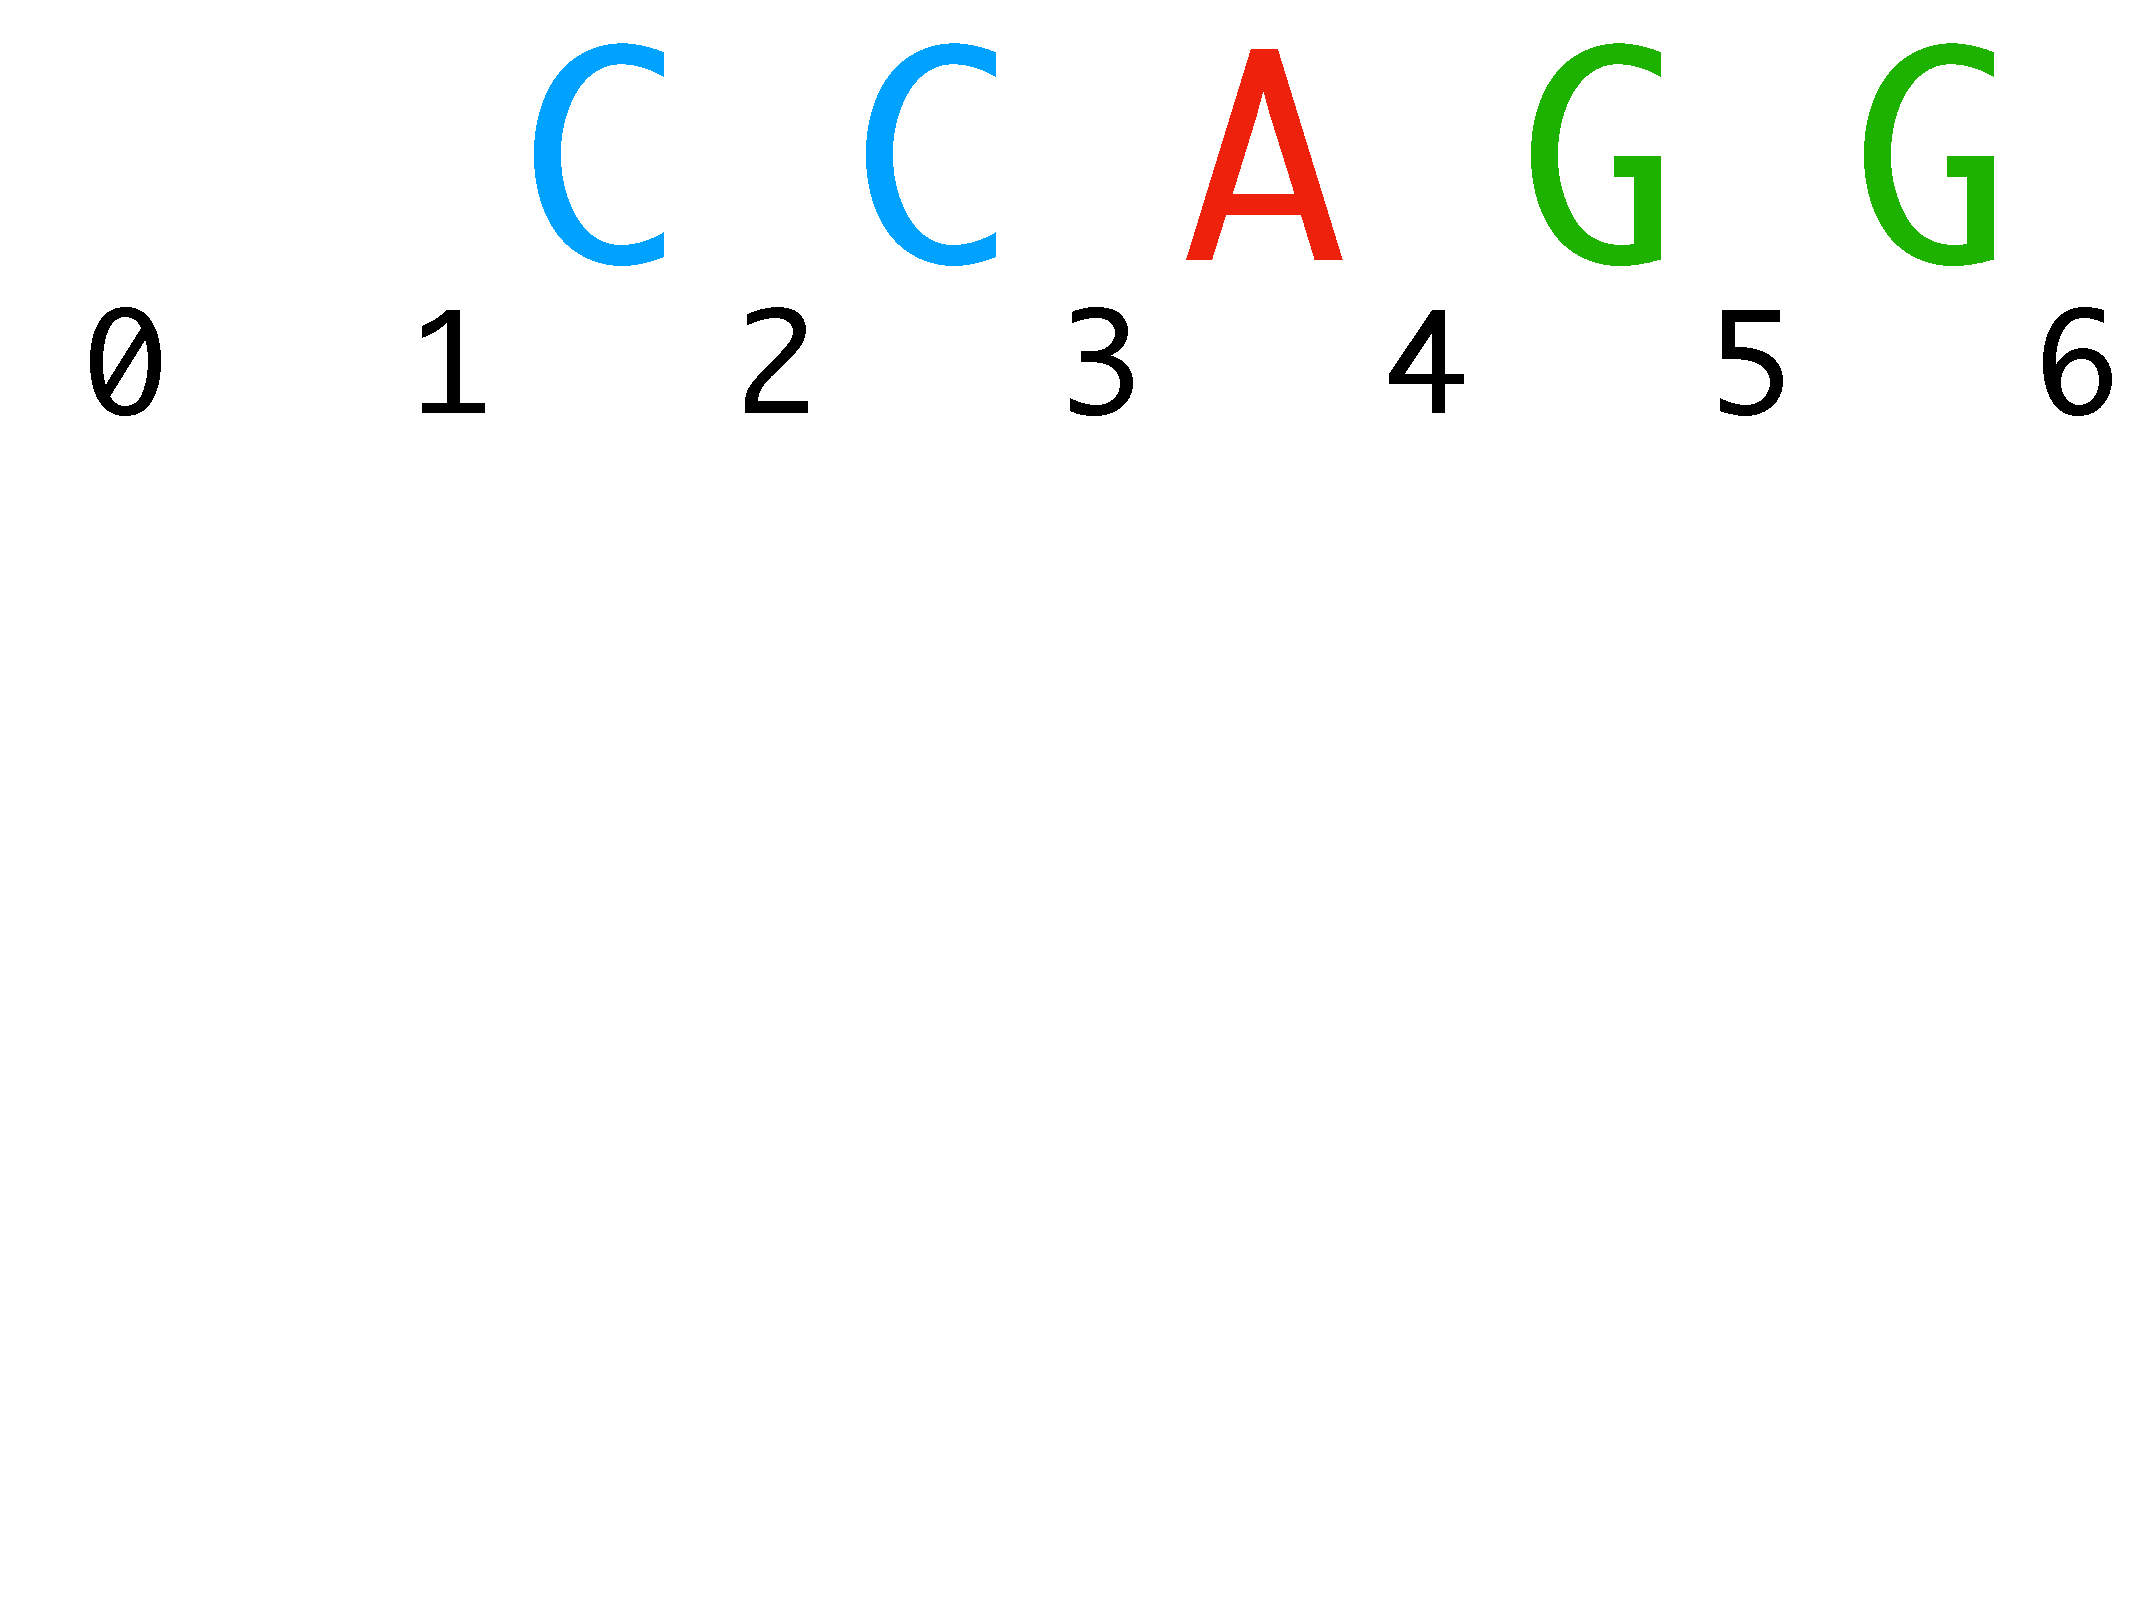
\includegraphics[scale=.16]{figs/index} \\[-3.cm]
%\hspace{-0.23cm}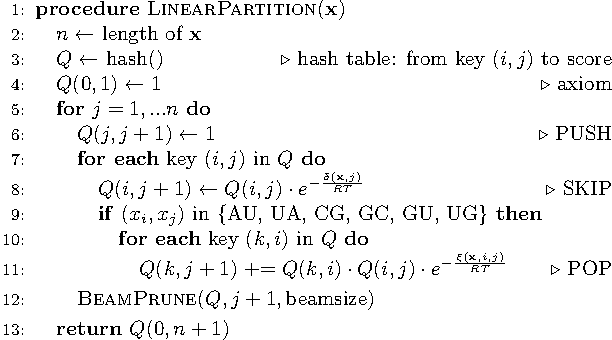
\includegraphics[scale=.83]{figs/algorithm} \\[0.2cm]
\begin{algorithmic}[1]
  \newcommand{\INDSTATE}[1][1]{\State\hspace{#1\algorithmicindent}}
  \setstretch{1.05} % lhuang: usepackage setspace
\Function{LinearPartition}{$\vecx, b$} \Comment{$b$ is the beam size}
% \bindent
    \State $n \gets$ length of $\mathbf x$
    \State $Q \gets$ hash() \Comment{hash table: from span $[i,j]$ to $\Qf{i}{j}$}
    \State $\Qf{j}{j-1} \gets 1$ for all $j$ in $1...n$ \Comment{base cases} \label{line:base}
    \For{$j=1 ... n$}
    \ForEach {$i$ such that $[i,\,j-1]$ in $Q$} \Comment{$O(b)$ iterations}
        \smallskip 
            \State $\Qf{i}{j} \pluseq \Qf{i}{j-1} \cdot e^{-\frac{\delta(\vecx,j)}{RT}} $ \Comment{\nskip} \label{line:skip}
            \If{$x_{i-1}x_j$ in \{AU, UA, CG, GC, GU, UG\}}  \label{line:pair}
                % \State $Q_{i,\,j+1} \gets  C(i,\,j) \cdot e^{-\frac{\xi(\vecx,i,\,j)}{RT}} $
                \ForEach{$k$ such that $[k,\,i-2]$ in $Q$} \Comment{$O(b)$ iters} \smallskip 
                    \State $\Qf{k}{j} \pluseq {\Qf{k}{i-2} \cdot \Qf{i}{j-1} \cdot e^{-\frac{\xi(\vecx,i-1,j)}{RT}}} $ \Comment{\pop} \label{line:pop}
                    % \State $C(0,j+1) \pluseq {C(0,k) \cdot C(k,j+1) \cdot e^{-\frac{\xi(\vecx,i,\,j)}{RT}}} $
                \EndFor
                % \State $C(0,j+1) \pluseq C(0,i) \cdot Q_{i,j+1}$ \Comment{COMBINE}
            \EndIf
        \EndFor
        \State $\textsc {BeamPrune}(Q,j, b)$ \Comment{choose top $b$ out of $Q(\cdot,j)$} \label{line:beamprune}%{see Fig.~\ref{fig:beam_prune_alg}}
        \EndFor
        \vspace{-0.1cm}
    \State \Return $Q$ \Comment{partition function $Q(\vecx)=\Qf{1}{n}$}
% \eindent
\EndFunction
\end{algorithmic}
% \end{algorithm}
\caption{
Partition function calculation pseudocode of a simplified version of the \linearpartition %linear-time partition function calculation
algorithm (the inside phase).
See Fig.~\ref{fig:beam_prune_alg} for the pseudocode of beam pruning (line~\ref{line:beamprune}).
The base-pairing probabilities are computed with the combination of the outside phase
(Fig.~\ref{fig:outside}).
% as well as a beam prune algorithm. 
% Here we model hash tables following Python dictionaries, where $(i, j) \in C$ checks whether the key $(i, j)$ is in the hash $C$; 
% this is needed to ensure linear runtime. 
% Quick select algotithm is used in beam prune, 
% and we skip the details for quick select here since it is well known.
% Real \linearpartition system is much more involved, but the pseudocode illustrates the left-to-right partition function calculation idea using a Nussinov-like fashion.
The actual algorithm using the Turner model is available on \href{https://github.com/LinearFold/LinearPartition}{GitHub}.
%See Fig.~\ref{fig:beam_prune_alg} for {\sc BEAMPRUNE} function.
\label{fig:algorithm}}
\vspace{-.3cm}
% \end{figure*}
\end{figure}


For simplicity of presentation,
in the pseudocode in Fig.~\ref{fig:algorithm}, $Q$ is notated as a hash table,
mapping from  $[i,j]$ to %its partition function
$\Qf{i}{j}$;
see Supplementary Information Section~\ref{sec:si:algdetails} for details
of its efficient implementation. % to make sure the overall runtime is $O(nb^2)$.
As the base case, we set $\Qf{j}{j-1}$ to be 1 for all $j$,
meaning all empty spans have partition function of 1 (line~\ref{line:base}).
%% %to store and look up states.   
%% $\langle 0,1 \rangle:1.0$ represents the dummy head state, 
%% whose partition function $Q(0,1)$ is initialized with value $1$.
%% This represents a structure with no pairs, 
%% i.e., the random coil, 
%% which is the reference state (free energy change of 0) and thus has equilibrium constant of 1.
%% {\color{blue}?????? (added by Mathews, but state <0,1>:1 is a singleton not a coil)}
Our algorithm then scans the sequence from left-to-right (i.e., from 5'-to-3'),
and at each nucleotide $x_j$ ($j=1...n$), % (the length of the sequence), 
% state $\langle 0,j+1 \rangle$ can always be extended with ``\md'' from state $\langle 0,j \rangle$.
% with its 
% Then we define three actions, PUSH, SKIP and POP
% to search states $\langle \cdot,j+1 \rangle$:
we perform two actions: %, \nskip and \pop:
%three actions, PUSH, SKIP and POP, are performed:
% similar as in \linearfold but different 
\begin{itemize}
%% \item PUSH: create a new state $\langle j,j \rangle:1$ representing an open bracket at $j$,
%% whose partition function is 1. 

%% 	% \begin{equation*}
%% 	% 	\frac{\langle i,j \rangle : \Qf{i,j]}{\langle j,j+1 \rangle : 1.0}
%% 	% \end{equation*}

\item \nskip (line~\ref{line:skip}): We extend each %state $[i,\,j-1]: \Qf{i,\,j-1]$ to a new state $[i,j]: \Qf{i,j]$
span $[i,\,j\!-\!1]$ in $Q$ to $[i,j]$ %: \Qf{i,j]$
by adding an unpaired base $y_j\!=$``\md'' (in the dot-bracket notation) to the right of each substructure in $\Qf{i}{j-1}$,
updating $\Qf{i}{j}$: % as follows:
\[
\Qf{i}{j} \pluseq \Qf{i}{j-1} \cdot e^{-\frac{\delta(\vecx, j)}{RT}}
\]
which can be visualized as
%\begin{center}
%  \vspace{-0.7cm}
%  \qquad \qquad
  \begin{tabular}{lr@{\,\quad}} % adjust alignment with j
    \multicolumn{2}{c}{
      $\overbrace{\myboxmath{\ \ \Qf{i}{j-1} \ \ } \ \Huge\md\!\!\!\!}^{\Qf{i}{j}}$
    }
    \\
    $i$ & $j$
  \end{tabular}.
%\end{center}
%% \begin{center}
%%   {

%%     \begin{tabular}{@{}l@{\;}c@{}}
%%       %      \hline
%%       \multicolumn{2}{c}{$\Qf{i,j]$}\\[0.1cm]
%%       \hline
%%   \myboxmath{\quad \Qf{i,j-1]\quad} & {\large\md} \\
%% %  \hline
%%    \multicolumn{1}{l}{$i$} & $j$
%%     \end{tabular}
%% }
%% \end{center}



	% \begin{equation*}
	% 	\frac{\langle i,j \rangle : \Qf{i,j]}{\langle i,j+1 \rangle : \Qf{i,j] \cdot e^{-\frac{\delta(\vecx, j)}{RT}}}
	% \end{equation*}
\vspace{-0.2cm}
\item \pop (lines~\ref{line:pair}--\ref{line:pop}): If $x_{i-1}$ and $x_j$ are pairable,
we combine span $[i,j-1]$ in $Q$ %[i,j]$ 
with each combinable ``left'' span $[k,i-2]$ in $Q$ %: \Qf{k,i-1]$,
% and create a new state $\langle k,j \rangle:Q(k,j)$,
% where $Q(k,j+1)=Q(k,i) \cdot \Qf{i,j] \cdot e^{-\frac{\xi(\vecx, i, j)}{RT}}$.
and update the resulting span $[k,j]$'s partition function % $[k,j+1]: Q(k,j+1)$
%as follows: 
\[
\Qf{k}{j} \pluseq \Qf{k}{i-2} \cdot \Qf{i}{j-1} \cdot e^{-\frac{\xi(\vecx, i-1, j)}{RT}}.
\]
This means that every substructure in $\Qf{i}{j-1}$ can be combined
with every substructure in $\Qf{k}{i-2}$ and a base pair $(i-1, j)$
to form one possible substructure in $\Qf{k}{j}$:
\begin{center}
  \vspace{-0.4cm}
  \begin{tabular}{l@{}r@{}l@{}r@{\,\quad}} %adjust alignment with j
    \multicolumn{4}{c}      
                {$\overbrace{\myboxmath{\; \Qf{k}{i-2}\; } {\Large\ml} \;\; \myboxmath{\; \Qf{i}{j-1}\; } \; {\Large\mr}}^{\Qf{k}{j}}$} \\
  $k$ \hspace{1.15cm} & $i\!-\!1$ & \hspace{0.02cm} {$i$} &  $j$
\end{tabular}
\end{center}
%% \begin{center}
%% \begin{tabular}{l@{}c@{\;}l@{\;}c}
%%   {\myboxmath{\; \Qf{k,i-1]\; }} & \ml & \myboxmath{\quad \Qf{i,j]\quad} & \mr \\
%%   {$x_k$} & $x_{i-1}$ & {$x_i$} & $x_j$
%% \end{tabular}
%% \end{center}

	% \begin{equation*}
	% 	\frac{\langle k,i \rangle : Q(k,i) \ \ \ \ \ \langle i,j \rangle : \Qf{i,j]}{\langle k,j+1 \rangle : Q(k,i) \cdot \Qf{i,j] \cdot e^{-\frac{\xi(\vecx, i, j)}{RT}}}
	% \end{equation*}

% Note that the operator of updating $Q(k,j+1)$ is "+=" (see Figure~\ref{algorithm} line 11).

% \item COMBINE: for each close state $\langle i,j \rangle$, it can be combined with its prefix state $\langle 0,i \rangle$ and form state $\langle 0,j+1 \rangle$:
% 	\begin{equation*}
% 		\frac{\langle 0,i \rangle : Q_{0,i} \ \ \langle i,j \rangle : Q_{i,j}}{\langle 0,j+1 \rangle : Q_{0,i} \cdot Q_{i,j} \cdot e^{-\frac{\xi(\vecx, i, j)}{RT}}}
% 	\end{equation*}
\end{itemize}

Above we presented a simplified version of our left-to-right \linearpartition algorithm. % that resembles \linearfold\/ {\em without} beam pruning.
%Like \linearfold,
We have 
three nested loops, one for $j$, one for $i$, and one for $k$,
and each loop takes at most $n$ iterations; % (i.e., $k,i$ and $j$ are all bounded by $n$).
therefore, the time complexity {\em without} beam pruning is $O(n^3)$,
which is identical to the classical McCaskill Algorithm (see Fig.~\ref{fig:overview}D).
In fact, there is an alternative, bottom-up, interpretation of our left-to-right algorithm
that resembles the Nussinov-style recursion of the classical McCaskill Algorithm:
\vspace{-0.1cm}
\[
\Qf{k}{j} \!=\! \Qf{k}{j-1} \cdot e^{-\frac{\delta(\vecx, j)}{RT}} + \!\! \sum_{k<i\leq j} \!\! {\Qf{k}{i-2} \cdot \Qf{i}{j-1}   \cdot e^{-\frac{\xi(\vecx, i-1, j)}{RT}}}
\]
%% \begin{equation*}
%% 	\begin{split}
%% 		\Qf{k}{j} &= \Qf{k}{j-1} \cdot e^{-\frac{\delta(\vecx, j)}{RT}} \\
%% 		       &+ \sum_{k<i\leq j} {\Qf{k}{i-2} \cdot \Qf{i}{j-1}   \cdot e^{-\frac{\xi(\vecx, i-1, j)}{RT}}}
%% 	\end{split}
%% \end{equation*}



%% % beam prune
%% The pseudocode in Figure~\ref{fig:algorithm} shows that our \linearpartition algorithm has three nested loops, 
%% one for $j$, one for $i$, and one for $k$,
%% and each loop has at most $n$ iterations. % (i.e., $k,i$ and $j$ are all bounded by $n$).
%% Therefore, the  time complexity without beam pruning is $O(n^3)$, which is identical to the classical McCaskill Algorithm,
However, unlike the classical bottom-up McCaskill algorithm,
our left-to-right dynamic programming, inspired by \linearfold, % instead of bottom-up fashion;
%% this is similar to the $O(n^3)$ left-to-right dynamic programming algorithm in \linearfold.
%% This left-to-right dynamic programming
makes it possible to further apply the beam pruning heuristic
%a heuristic method,
to achieve linear runtime in practice.
% and achive linear runtime.
The main idea is, at each step $j$, among all possible spans $[i, j]$ that ends at $j$  (with $i=1...j$), 
we only keep the top $b$ most promising candidates (ranked by their partition functions \Qf{i}{j}).
%i.e., the top $b$ among all \Qf{i}{j}'s,
%those %$(i,j)$
%with higher partition functions, %value $Q_{i,j}$, 
%and remove the other ones
where $b$ is the beam size.
% We adopt quick select algorithm to ensure the process of selecting top $b$  candidates costs linear runtime.
With such beam pruning, 
we reduce the number of states from $O(n^2)$ to $O(nb)$,
and the runtime from $O(n^3)$ to $O(nb^2)$.
For details of the efficient implementation and runtime analysis, please refer to
Supplementary Information Section~\ref{sec:si:algdetails}.
Note $b$ is a user-adjustable constant ($b=$100 by default).


After the partition-function calculation, also known as the ``inside'' phase of the classical inside-outside algorithm~\cite{baker:1979},
we design a similar linear-time ``outside'' phase (see Supplementary Section~\ref{sec:outside})
to compute the base pairing probabilities:
\vspace{-0.1cm}
\[
p_{i,j} = \sum_{(i,j)\in \pairs(\vecy)} p(\vecy),
\]
where $p_{i,j}$ is the probability of nucleotide $i$ pairing with $j$,
which sums the probabilities of all structures that contain $(i,j)$ pair,
and $p(\vecy)=e^{-\frac{\Delta G^\circ(\vecy)}{RT}} / Q(\vecx)$
is the probability of structure \vecy % of the structure $\vecy$ in the ensemble.
in the ensemble.  %among all possible structures
%(or the probability of $i$ being unpaired when $j=N+1$).



